\documentclass[a4paper,12pt]{article}
\usepackage{amsmath,amssymb,amsfonts,amsthm}
\usepackage{tikz}
\usepackage [utf8x] {inputenc}
\usepackage [T2A] {fontenc} 
\usepackage[russian]{babel}
\usepackage{cmap} 
\usepackage{ gensymb }
% Так ссылки в PDF будут активны
\usepackage[unicode]{hyperref}
\usepackage{ textcomp }

% вы сможете вставлять картинки командой \includegraphics[width=0.7\textwidth]{ИМЯ ФАЙЛА}
% получается подключать, как минимум, файлы .pdf, .jpg, .png.
\usepackage{graphicx}
% Если вы хотите явно указать поля:
\usepackage[margin=1in]{geometry}
% Или если вы хотите задать поля менее явно (чем больше DIV, тем больше места под текст):
% \usepackage[DIV=10]{typearea}

\usepackage{fancyhdr}

\newcommand{\bbR}{\mathbb R}%теперь вместо длинной команды \mathbb R (множество вещественных чисел) можно писать короткую запись \bbR. Вместо \bbR вы можете вписать любую строчку букв, которая начинается с '\'.
\newcommand{\eps}{\varepsilon}
\newcommand{\bbN}{\mathbb N}
\newcommand{\dif}{\mathrm{d}}

\newtheorem{Def}{Определение}


\pagestyle{fancy}
\makeatletter % сделать "@" "буквой", а не "спецсимволом" - можно использовать "служебные" команды, содержащие @ в названии
\fancyhead[L]{\footnotesize Оптика}%Это будет написано вверху страницы слева
\fancyhead[R]{\footnotesize ФМХФ МФТИ}
\fancyfoot[L]{\footnotesize \@author}%имя автора будет написано внизу страницы слева
\fancyfoot[R]{\thepage}%номер страницы —- внизу справа
\fancyfoot[C]{}%по центру внизу страницы пусто

\renewcommand{\maketitle}{%
	\noindent{\bfseries\scshape\large\@title\ \mdseries\upshape}\par
	\noindent {\large\itshape\@author}
	\vskip 2ex}
\makeatother
\def\dd#1#2{\frac{\partial#1}{\partial#2}}


\title{4.7.2 \\ Эффект Поккельса}
\author{Егор Берсенев} 
\date{16 февраля 2017 г.}

\begin{document}
	\maketitle
	\section{Цель работы}
		Исследовать интерференцию рассеянного света, прошедшего кристалл; наблюдать изменение характера поляризации света при наложении на кристалл электрического поля.
	\section{Оборудование}
	Гелий-неоновый лазер, поляризатор, кристалл $\text{LiNbO}_3$, матовая пластинка, экран, источник высоковольтного переменного напряжения, фотодиод, осциллограф, линейка.
	
	\section{Теоретическое введение}
	
	В одноосных кристаллах существует два типа монохроматических волн, называемых обыкновенными и необыкновенными. Вектор $\boldsymbol{D}$ обыкновенной волны перпендикулярен плоскости оптической оси кристалла и волнового вектора: $\boldsymbol{D} = \varepsilon_{\bot}\boldsymbol{E}_{\bot}$. Вектор $\boldsymbol{D}$ необыкновенной волны лежит в главном сечении: $\boldsymbol{D} = \varepsilon_{\bot}\boldsymbol{E}_{\bot} + \varepsilon_{\|}\boldsymbol{E}_{\|}$.  
	
	\begin{figure}[h!]\label{fig:unusual}
		\begin{center}
			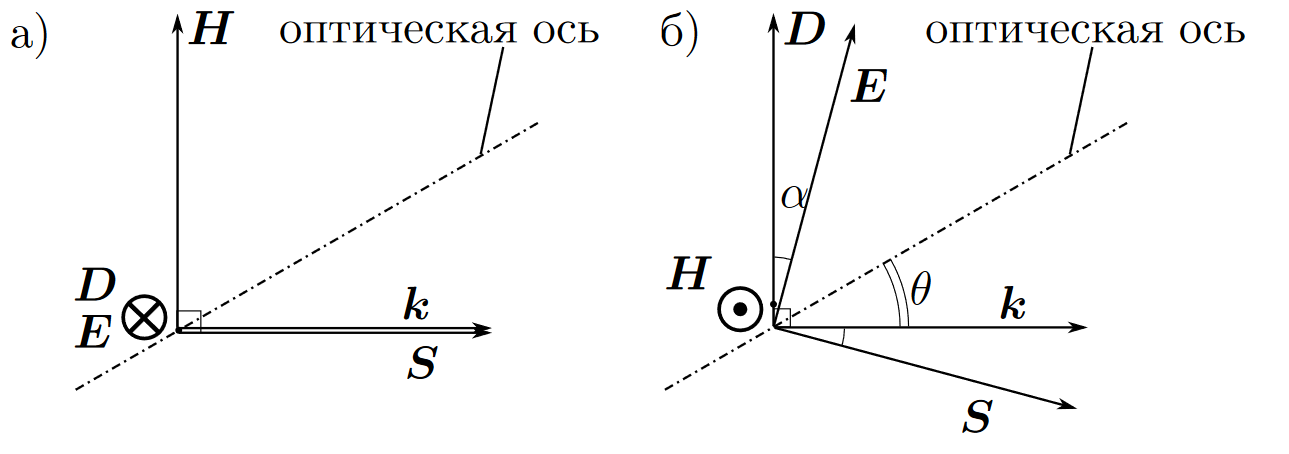
\includegraphics[width=0.8\linewidth]{unusual}
			\caption{а) обыкновенная и б) необыкновенные волны}
		\end{center}
	\end{figure}
	
	\begin{equation}\label{eq:prelom}
	\left\{
	\begin{aligned}
	& n_0 = \sqrt{\varepsilon_{\bot}} \text{, обыкновенная волна} \\
	& n(\theta) = \left(\frac{\sin^2(\theta)}{\varepsilon_{\|}} + \frac{\cos^2(\theta)}{\varepsilon_{\bot}}\right)^{-1/2} \text{, необыкновенная волна}
	\end{aligned}
	\right.
	\end{equation}
	
	\begin{figure}[h!]\label{fig:interferention}
		\begin{center}
			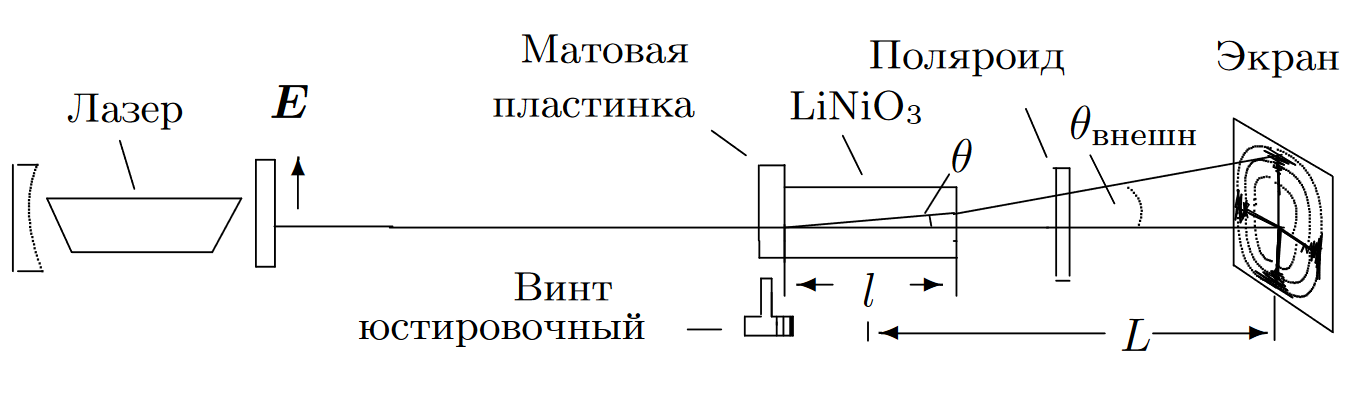
\includegraphics[width=0.8\linewidth]{interferention_scheme}
			\caption{Схема для наблюдения интерференционной картины}
		\end{center}
	\end{figure}
	
	Эффектом Поккельса называется изменение показателя преломления света в кристалле под действием электрического поля. При отсутствии внешнего электрического поля разность хода между обыкновенной и необыкновенной волнами при прохождении через кристалл длиной $l$ равна: \[\Delta\varphi = \frac{2\pi}{\lambda}l(n_1 - n_2) \]
	Для обыкновенного луча $n_1 = n_0$, для необыкновенного луча, считая что $n_e = \sqrt{\varepsilon_{\|}}$ и $n_0$ отличаются незначительно и угол $\theta$ малый (см. равенство \eqref{eq:prelom}): \[n_2 \approx n_0 - (n_0 - n_e)\theta^2\]
	Тогда \[\Delta\varphi = \frac{2\pi}{\lambda}l(n_0 - n_e)\theta^2\]
	Интерференционная картина представляет собой концентрические окружности. Для m-го темного кольца $\Delta\varphi = 2\pi m$. Если $L$ - расстояние от центра кристалла до экрана, то, учитывая закон преломления на границе кристалла, при малых углах $\theta_{\text{внешн.}} = n_0\theta$ (рис. \ref{fig:interferention}) получаем выражение для радиуса кольца:
	
	\begin{equation}\label{eq:radius}
	r_m^2 = \frac{\lambda}{l}\frac{(n_0L)^2}{(n_0 - n_e)}m
	\end{equation}  
	
	При наличии внешнего электрического напряжения появляется разность фаз \[\Delta\varphi = \frac{2\pi}{\lambda}\frac{l}{d}AU\text{,}\] где $U$ - напряжение на кристалле, $d$ - размер кристалла в поперечном направлении, $A$ - константа, зависящая от типа кристалла.
	
	\vspace{\baselineskip}
	
	При перпендикулярной и параллельной поляризациях лазера и анализатора интенсивность света на выходе определяется выражениями:
	\begin{equation}\label{eq:intensity}
	\begin{aligned}
	&I_{\text{вых}\bot} = I_0\sin^2\left(\frac{\pi}{2}\frac{U}{U_{\lambda/2}}\right)\\
	&I_{\text{вых}\|} = I_0\cos^2\left(\frac{\pi}{2}\frac{U}{U_{\lambda/2}}\right) 
	\end{aligned}
	\end{equation} 
	
	Где
	\begin{equation}\label{eq:half_lambda}
	U_{\lambda/2} = \frac{\lambda}{4A}\frac{d}{l}
	\end{equation} - полуволновое напряжение, т.е. при разности хода $\lambda/2$ $I_{\text{вых}\bot}$ достигает максимума.
	
	\section{Экспериментальная установка}
	
	В нашем эксперименте $L = 82 \pm 5 cm$, $n_0 = 2.29$, $\lambda = 0.63 \mu m$\\ Размеры кристалла: $3\times3\times26$
	
	\begin{figure}[h!]\label{fig:experiment}
		\begin{center}
			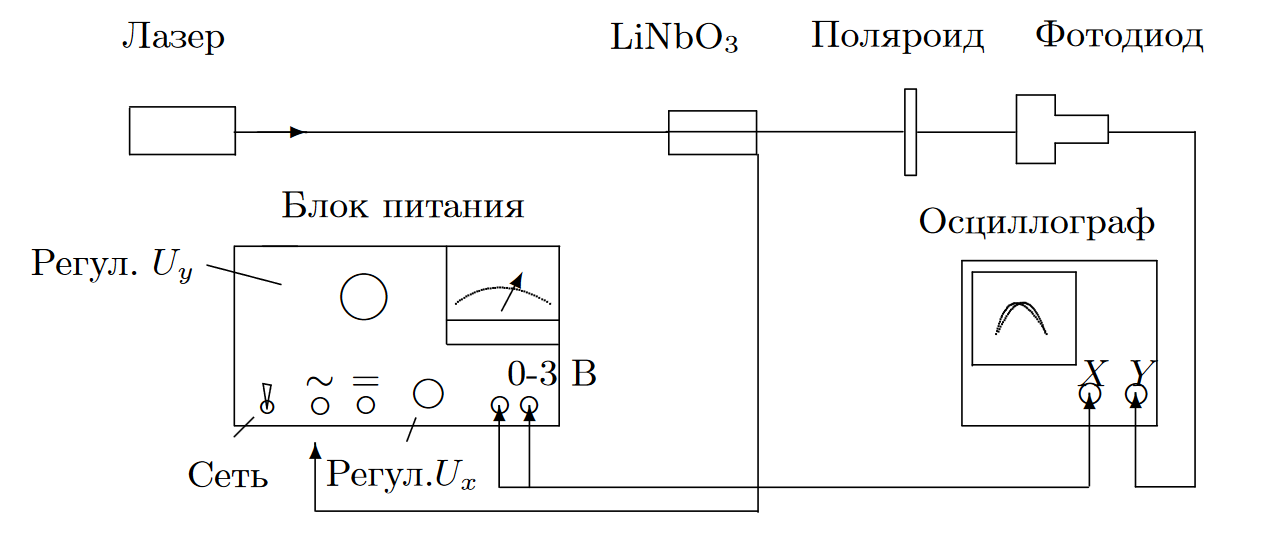
\includegraphics[width=0.8\linewidth]{experiment_scheme}
			\caption{Схема экспериментальной установки}
		\end{center}
	\end{figure}
	

	\section{Экспериментальная часть}
		
		Измерим радиусы темных колец интерференционной картины(таблица ). Построим график $r^2 = f(m)$ и по углу наклона прямой определим двулучепреломление $(n_0 - n_e)$ ниобата лития.
		
		\begin{table}[h!]\label{tab:radius}
			\centering
			\caption{Радиусы темных колец}
			\resizebox{\textwidth}{!}{%
				\begin{tabular}{|c|c|c|c|c|c|c|c|c|c|c|c|}
					\hline
					n      & 1   & 2    & 3   & 4   & 5   & 6   & 7   & 8   & 9   & 10  & 11  \\ \hline
					$r_n$, cm & 3.1 & 4.15 & 5.0 & 5.8 & 6.5 & 7.2 & 7.8 & 8.3 & 8.8 & 9.2 & 9.6 \\ \hline
				\end{tabular}%
			}
		\end{table}
		
		\begin{figure}[h!]\label{fig:radius}
			\begin{center}
				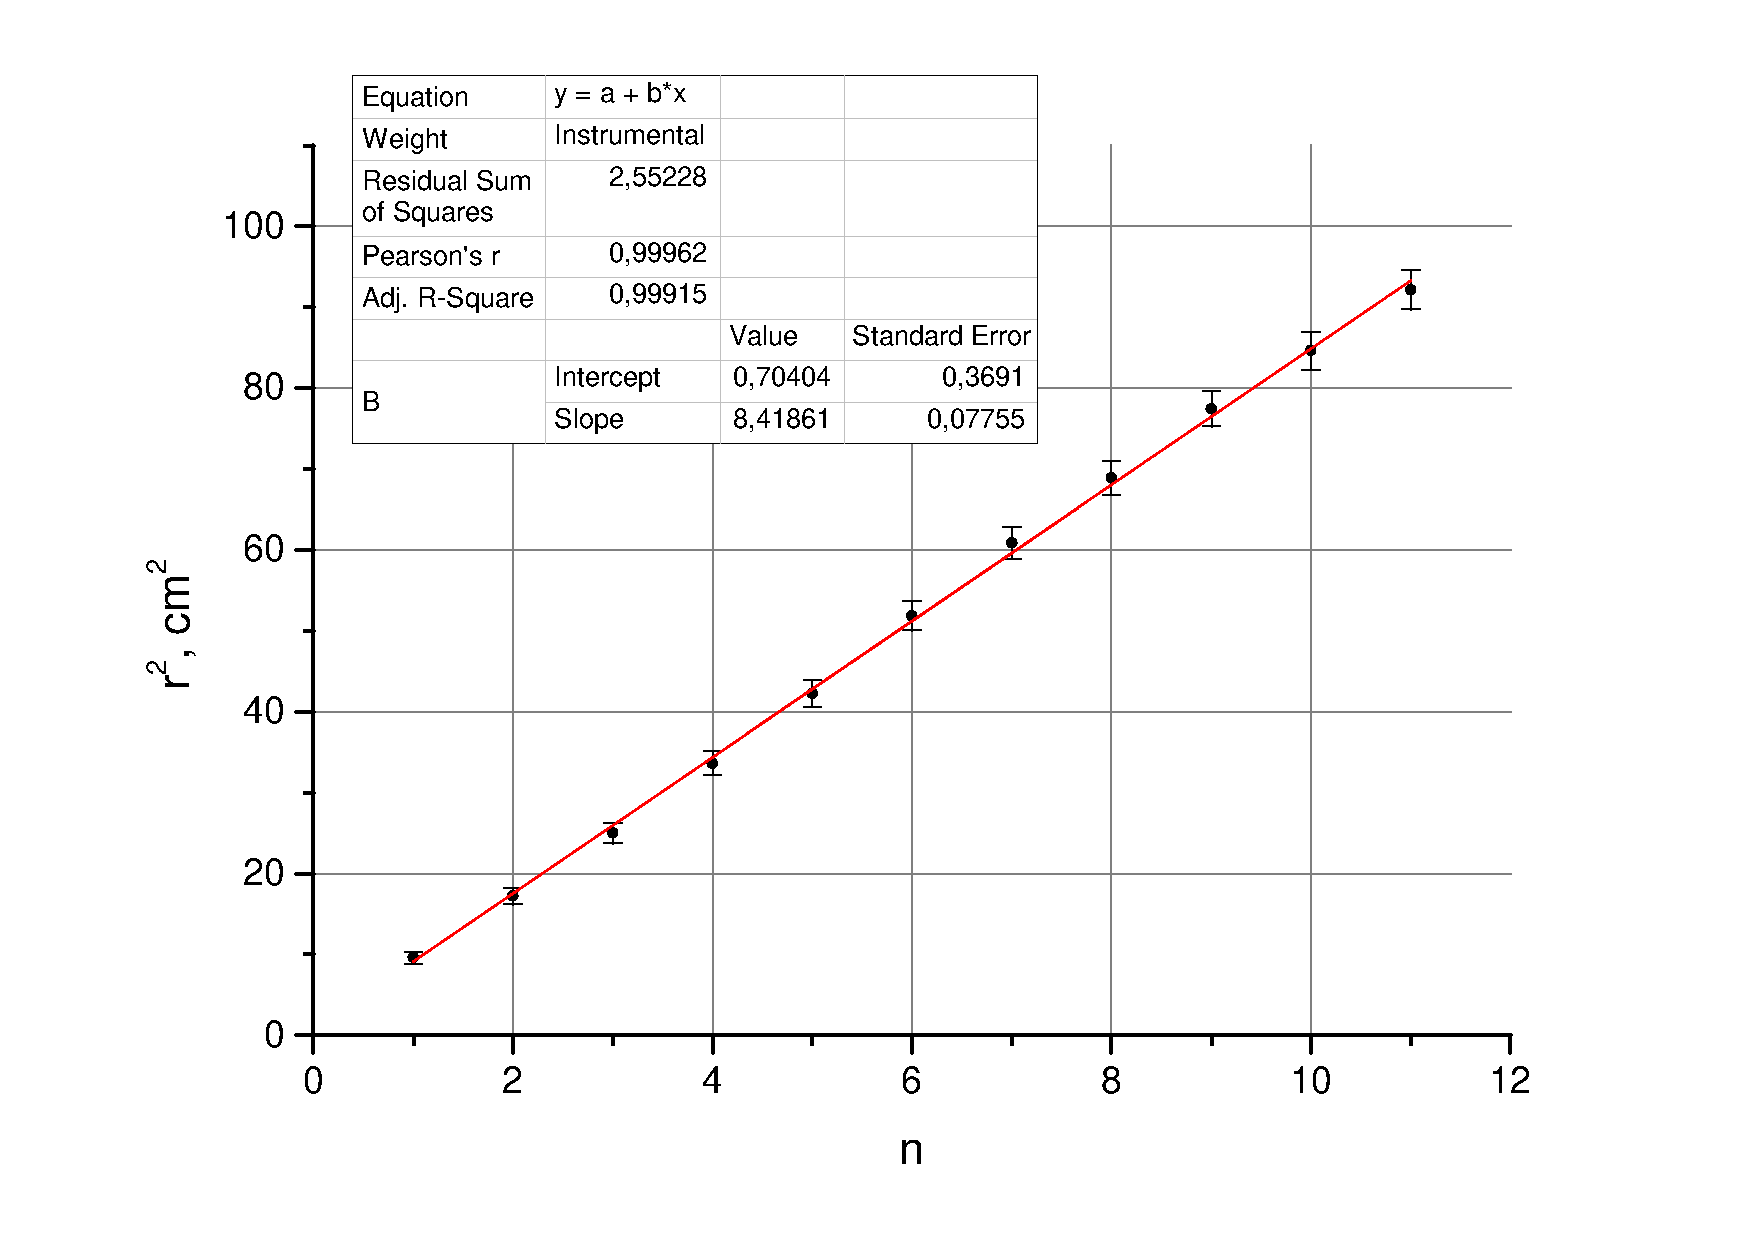
\includegraphics[scale=0.5]{graph}
				\caption{График зависимости $r_m$ от номера кольца}
			\end{center}
		\end{figure}
		
		$$ k = \frac{\lambda}{l}\frac{(n_0L)^2}{(n_0 - n_e)} = 8.41\pm0.08\text{ cm}^2 \Rightarrow n_0 - n_e = 0.10\pm0.01 $$
		
		Подадим на кристалл постоянное напряжение и определим по максимуму яркости пятна на экране:$$ U_{\lambda/2} = 0.45\pm0.03 \text{ кВ}$$
		
		Подадим на кристалл напряжение $U = U_{\lambda/4} = 0.5U_{\lambda/2}$ и, вращая поляризатор, убедимся в круговой поляризации света(яркость пятна практически не меняется).
		
		
		Установим вместо экрана фотодиод, переключим напряжение с постоянного на переменное и пронаблюдаем фигуры Лиссажу на экране осциллографа при плавном изменении напряжения. Первый максимум сигнала на осциллограмме соответствует напряжению:$$ U_{\lambda/2~} = 0.45\pm0.03\text{ кВ}$$
		
		\begin{figure}[h!]
			\begin{center}
				\begin{minipage}{0.3\textwidth}
					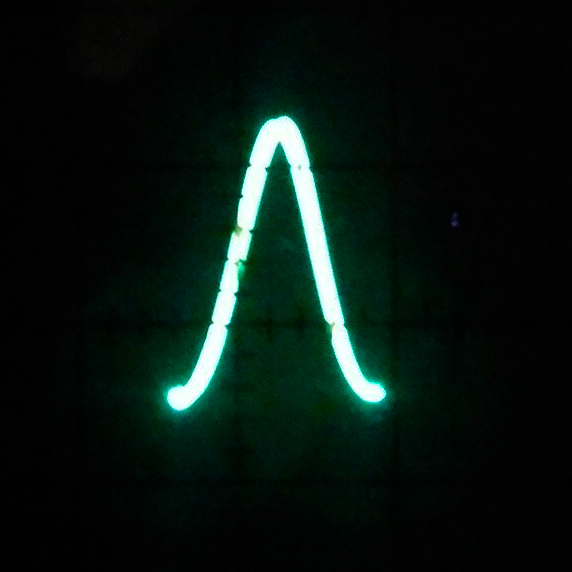
\includegraphics[width=\textwidth]{one}
					\caption{$U = U_{\lambda/2}$}
				\end{minipage}
				\hfill
				\begin{minipage}{0.3\textwidth}
					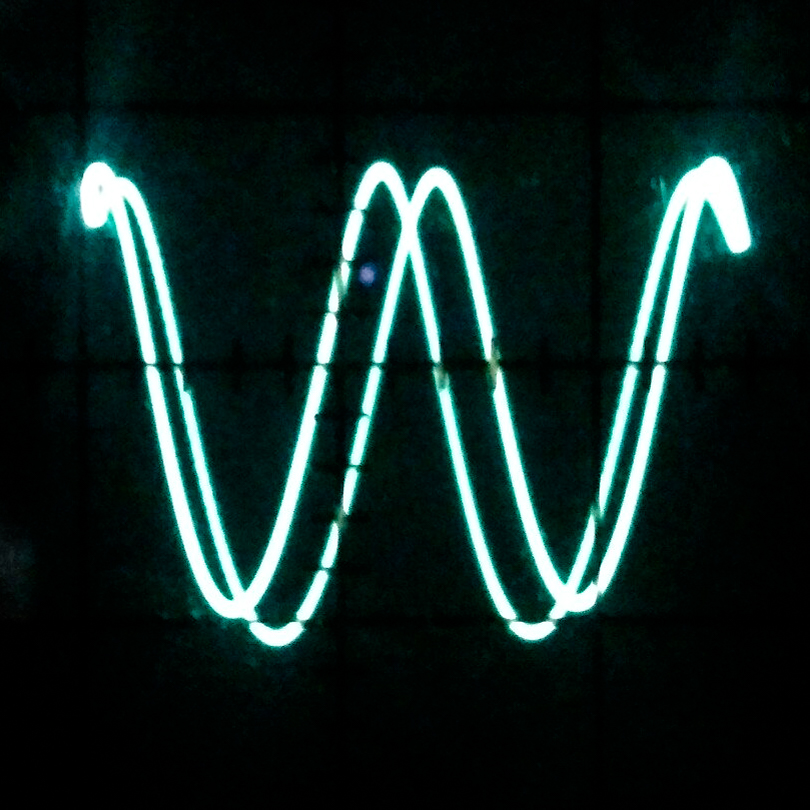
\includegraphics[width=\textwidth]{two}
					\caption{$U = 2U_{\lambda/2}$}
				\end{minipage}
				\hfill
				\begin{minipage}{0.3\textwidth}
					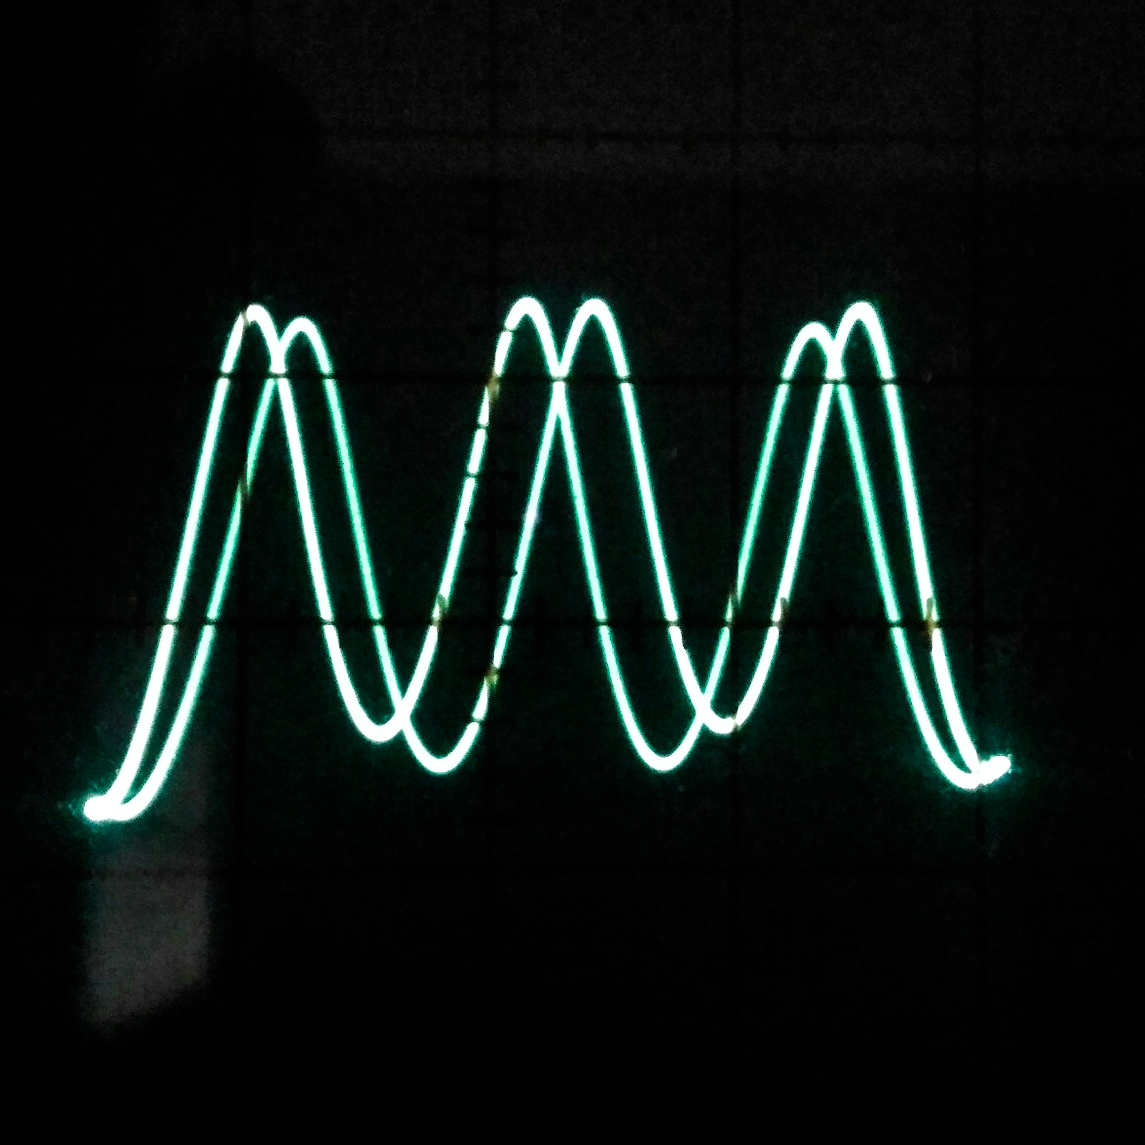
\includegraphics[width=\textwidth]{three}
					\caption{$U = 3/2U_{\lambda/2}$}
				\end{minipage}
			\end{center}
		\end{figure}
		
		\section{Вывод}
		
		В проделанной работе была изучена интерференционная картина рассеянного света, пропущенного через кристалл. Также был исследован характер зависимости поляризации света при наложении на кристалл электрического поля.
	

	
\end{document}


